% Chapter Template

\chapter{Deep Learning} % Main chapter title

\label{Chapter4} % Change X to a consecutive number; for referencing this chapter elsewhere, use \ref{ChapterX}

The chapter is inspired by \parencite{Goodfellow-et-al-2016,Mackay18} which the interested reader can find more information about deep learning. Deep learning experiences a renaissance, because of the technology improvements in hardware and software. The collection of data has also significant improved the field. Deep learning is a specialized field in machine learning, where you focus on a special architecture of models. Like in machine learning the basic components of a deep learning algorithm are a data set, cost function, optimization algorithm and a model. E.g. in the LSM method we assumed the linear model, data set was the simulated paths, the cost function was the mean square error and the optimization algorithm was a closed form solution of the normal equations. Deep learning is about studying neural networks which allows for greater flexibility than standard methods like linear regression. \\

A neural network consists of multiple layer, where the depth tells you how many layers the network has (see figure \ref{fig:multilayer-perceptron}), hence the name "Deep learning". All the algorithms applied will be within supervised learning, where we try to fit the best relationship between the features and the response variable. Furthermore all our algorithms will be based on the multilayer perceptrons (MLPs) for regression, therefore most of the chapter present the theory for supervised MLPs regression. The advantage of a multilayer model is that for each layer the updated set of covariates can be more finely tuned to better explain the data making the model extremely flexible. The MLPs is also called feedforward neural networks because the information only travels forward in the neural network, through the input node(s) then through the hidden layer(s) and finally through the output node(s). First we present the basics for machine learning and then specialize the theory to deep learning.

%----------------------------------------------------------------------------------------
%	SECTION 1
%----------------------------------------------------------------------------------------

\section{Machine Learning Basics}
The task for machine learning is to learn from data with respect to some performance measure. "A computer program is said to learn from experience E with respect to some class of tasks T and performance measure P, if its performance at tasks in T, as measured by P, improves with experience E" (\parencite{Goodfellow-et-al-2016} p. 97). Classical tasks T could be classification or regression, where the two methods differ on the output type. The former has discrete outputs, where regression has continuous output. We are interested finding a price, which is naturally represented as a continuous value hence our task will be to regress the price or continuation value like in LSM. Measuring performance depends on the task, but for regression a typical performance measure is mean squared error (MSE):
$$\frac{1}{K}\sum_{k=1}^{K} (y_k-\hat{y}_k)^2$$
There are other methods for measuring performance e.g. mean absolute error (MAE). Another measure to quantify the fit is coefficient of determination:
$$R^2=1-\frac{\frac{1}{K}\sum_{k=1}^{K} (y_k-\hat{y}_k)^2}{\frac{1}{K}\sum_{k=1}^{K} (y_k-\bar{y})^2} \quad \text{where $\bar{y}$ is the sample mean}$$
Coefficient of determination explains how well the model explains the data compared to the empirical mean. Some care should be taken by comparing models with different capacity, because the coefficient of determination will tend to prefer the larger models. The experience comes from data, where the data can be given with or without target values $\bm{y}$. In machine learning the task is quite different depending on targets are given or not, hence the algorithms are split into two categories; supervised and unsupervised learning. The terminology supervised comes from a teacher gives you the target values $\bm{y}$ that the algorithms tries to predict from $\matr{X}$.3\\

Machine learning is not about making overly complex models to fit your data perfectly, because then the model will most likely have poor performance on unseen data. This phenomenon is known as overfitting, but the models can also be too simple known as underfitting. If machine learning only cared about performance on the given data for training, then machine learning would be essentially optimization. The key difference is that machine learning wishes to obtain statistical generalization to unseen data. The practical way to evaluate the model is to measure generalization error on a test set. In machine learning the data is split into test data and training data, where the test set can only be used for evaluation after training. \\

The training data is used for training the model, where the training error tells how the fitted parameters fits to the training data. An unacceptable high training error could indicate the regression method could be too simple and underfitting is the issue. For training it can sometimes also be useful to have a validation data set to see how your model generalizes, because the test set cannot be used to make model choices, hence it is common to split the training set into a validation and training set. The validation set is allowed to be used in training and it tries to mimic the generalization error. A common technique for measuring validation errors is "cross-validation", where the data set is split into training and validation sets depending on the cross-validation scheme. The aim for the validation data is to approximate the model performance on unseen data, which is essentially what we want to be within an acceptable range.\\

After training the model we can evaluate the performance on a test set not seen in training. An unacceptable high test error when evaluating the model and very low training error could be an example of overfitting the model. Hence when training the model, we wish best of both worlds an acceptable training error and making the gap between training and test error acceptable as well. In machine learning the overfitting and underfitting concepts are expressed by the relation of bias-variance trade-off, where there is a trade-off between training error and generalization error. In case of overfitting the model has been extensively trained to get a low biases, but the trade-off is that the model does not generalize well represented by a high variance.\\

A technique known as regularization is one approach to avoid overfitting. The regularization term is added to the cost function $J(\theta)$, which is essentially the function to minimize in order to train the model. There is a lot different regularization methods, where in the MLPs section \ref{multilayerPerceptron} we will present some useful regularization for deep learning models. Besides the parameter estimated within the model, there is a need for model designs (hyperparameters).\\

Hyperparameter is the parameters not estimated within the model, but rather exogenous given values from the model designer. Some common examples in machine learning and deep learning is the learning rate, batch size, weight decay, model capacity, etc. The choice of the hyperparameters is often more important than the optimization algorithm chosen to estimate the parameters within the model, hence the need for suitable choices for hyperparameters is needed for most machine learning models. The calibration of the model to a specific task is called hyperparameter tuning, where it can be done manually or automatically. The manual choice requires expert knowledge to set the hyperparameter optimal for the given task, where the automatic procedures is often computational expensive. Examples of hyperparameters rutines are random search, grid search and Bayesian optimization.\\

The parameters within the model are found by minimizing the cost function $J(\theta)$. In some cases there exist either a closed form solution or the cost function is convex making the optimization problem easier to handle. The complexity of MLPs makes the cost function non convex and iterative optimization procedures are needed. The basic iterative procedure is the gradient descent where the concept is to repeatedly making small moves in parameters toward better configuration. The most popular gradient methods in deep learning are Adam, RMSProp, AdaGrad and stochastic gradient descent (SGD). The methods will be discussed in more details in section \ref{trainNetwork}. To sum up a machine learning model needs a data set, a model, a cost function and an optimization algorithm. Understanding of basic machine learning will be the foundation for deep learning.


%----------------------------------------------------------------------------------------
%	SECTION 2
%----------------------------------------------------------------------------------------

\section{Multilayer Perceptrons}\label{multilayerPerceptron}
The goal of the multilayer perceptrons (MLPs) is to approximate a function $f^*(x)$, where the MLPs defines a mapping $x\in \mathbb{R}^R \mapsto f(x;\theta)$ to approximate $f^*(x)$. The task is to find the best $\theta$ such that the approximation $f(x;\theta)$ is close to the targets measured by a defined cost function $J(\theta)$. With the minimized cost function the goal is to archive statistical generalization i.e. useful results for test data not used for training. \\

The first step for MLPs is building the network, where we start with zooming in on a single neuron, which is one node of a directed acyclic graph (figure \ref{fig:multilayer-perceptron}). Note that the MLPs is also called a feedforward network, because all the connections between the neurons are directed such that the network forms a directed acyclic graph.

%-----------------------------------
%	SUBSECTION 1
%-----------------------------------
\subsection{A Single Neuron}\label{singleNeuron}
The single neuron has a number $R$ features of inputs $x_r$ and one output $\hat{y}$ (see figure \ref{fig:singleNeuron}). 

\tikzset{%
  every neuron/.style={circle,draw,minimum size=1cm},
  neuron missing/.style={draw=none,scale=4,text height=0.333cm,execute at begin node=\color{black}$\vdots$},
}
\begin{center}
    \begin{figure}[h]
        \begin{tikzpicture}[
        		init/.style={
 				draw,
  				circle,
  				inner sep=2pt,
  				font=\Huge,
  				join = by -latex
			},
			squa/.style={
  				draw,
  				inner sep=2pt,
  				font=\Large,
  				join = by -latex
			},
			start chain=2,node distance=13mm
			]
			\node[on chain=2] 
			  (x2) {$x_2$};
			\node[on chain=2,join=by o-latex] 
			  {$w_2$};
			\node[on chain=2,init] (sigma) 
			  {$\displaystyle\Sigma$};
			\node[on chain=2,squa,label=above:{\parbox{2cm}{\centering Activate \\ function}}]   
			  {$g$};
			\node[on chain=2,label=above:Output,join=by -latex] 
			  {$y$};
			\begin{scope}[start chain=1]
			\node[on chain=1] at (0,1.5cm) 
 				(x1) {$x_1$};
			\node[on chain=1,join=by o-latex] 
				  (w1) {$w_1$};
			\end{scope}
			\begin{scope}[start chain=3]
				\node[on chain=3] at (0,-1.5cm) 
				  (x3) {$x_3$};
				\node[on chain=3,label=below:Weights,join=by o-latex] 
			 	 (w3) {$w_3$};
			\end{scope}
			\node[label=above:\parbox{2cm}{\centering Bias \\ $w_0$}] at (sigma|-w1) (b) {};

			\draw[-latex] (w1) -- (sigma);
			\draw[-latex] (w3) -- (sigma);
			\draw[o-latex] (b) -- (sigma);

			\draw[decorate,decoration={brace,mirror}] (x1.north west) -- node[left=10pt] {Inputs} 				(x3.south west);
        \end{tikzpicture}
        \caption{A single neuron}
        \label{fig:singleNeuron}
    \end{figure}
\end{center}



The function from inputs to output for a single neuron is:
\begin{align}   
\hat{y}=g(w_0 + \bm{x}^T \bm{w}) \quad where \quad \bm{x}=\begin{pmatrix}
x_1 \\
\vdots\\
x_R
\end{pmatrix} \quad and \quad \bm{w}=\begin{pmatrix}
w_1 \\
\vdots \\
w_R
\end{pmatrix}
\end{align}
The $\bm{w}$ is the weight matrix (this case a vector) and $w_0$ is the bias term. The term inside the function g is the activation of the neuron and it is a affine transformation denoted:
$$a= w_0 + \bm{x}^T \bm{w}$$
The function g is the activation function and it is essential for the flexibility of the MLPs. There exists numerous of activation functions only the imagination is the limit. We will list the most common and discuss them.


%-----------------------------------
%	SUBSUBSECTION 1
%-----------------------------------
\subsubsection{Activation functions}
Activation functions are essential for neural network, because they allow for non-linearities and flexibility. Activation functions apply a non-linear transformation and decide whether a neuron should be activated or not. Without activation functions or the activation function being the identity function $g(a)=a$ the whole network would essentially be a linear regression model. Some popular activation functions are:
\begin{enumerate}
\item[•] Sigmoid function: $g(a)=\frac{1}{1+\exp(-a)}$\\

This is the traditional choice, also called the logistic function. Popular in classification but can suffer from vanishing gradient in deep learning.
\item[•] Hyperbolic tangent function: $g(a)=\frac{e^a-e^{-a}}{e^a+e^{-a}}$\\

A scaled and shifted sigmoid function and likewise suffers from the vanishing gradient problem. The range is $(-1,1)$ and centered at zero. Often used for hidden layers.
\item[•] ReLU function: $g(a)=\max(0,a)$.\\

Rectified Linear Unit is one of the most popular choices since it does not suffer from the vanishing gradient problem. The MLPs often becomes more sparse because it sets some features to zero. It is claimed that ReLU learns multiple times faster than both the hyberbolic tangent and the sigmoid function.
\item[•] Leaky ReLU function:  \[ g(a)=
    \begin{dcases}
        a & if \ a \geq 0 \\
        \alpha \cdot a & otherwise \\
    \end{dcases}
\]\\
The fact that ReLU can have some hidden covariates that is zero which can be an advantage. A disadvantage of ReLU is some neurons may die out if the neurons are mapped to zero. The Leaky ReLU is designed to give such neurons a chance to get back into action, but not too easily, so $\alpha>0$ is chosen small ( typical $\alpha=0.01$ ) 

\item[•] ELU - exponential linear unit:  \[ g(a)=
    \begin{dcases}
        a & if \ a \geq 0 \\
        \alpha(\exp(a)-1) \cdot x & otherwise \\
    \end{dcases}
\]\\
Like the Leaky ReLU the ELU is designed to avoid the dead ReLU problem. 
\end{enumerate}

With a understanding of a single neuron we continue to the architecture of a MLPs.


%-----------------------------------
%	SUBSECTION 2
%-----------------------------------
\subsection{Architecture Of MLPs}\label{architectureMLPs}
A MLPs consists of a input layer, where all $R$ features enter, $L$ hidden layers, and an output layer. Each hidden layer and the output layer consists of multiple neurons, where the width of the layer is the number of neurons in that layer ($m^l$) (see figure \ref{fig:multilayer-perceptron}). The networks inputs are called the input layer, the output layer is the output of the neural network. The layers between the input and output layer are hidden layers. This could be an explanation why the field is called Deep learning, because of a deep structure of layers. In each hidden layer a linear combination of the features from the previous layer is made and then an activation function is applied in order to create the new hidden features in that layer (see figure \ref{fig:multilayer-perceptron}). The MLPs is essential a large nested function, where the input layer go through a chain of functions until reaching the output.
\begin{align}
\bm{f}(\bm{x};\bm{\theta})=\bm{f}_1 \circ \bm{f}_2 \circ \cdots \circ \bm{f}_{L+1}\\
where \ \bm{f}_i : \mathbf{R}^{m^{i-1}} \to \mathbf{R}^{m^{i}} \quad i=1,\ldots, L+1
\end{align}
Each function in the composition of functions corresponds to a layer of neurons.
\begin{align}
\bm{f}_i(x)=\bm{g}(\matr{W}^T \bm{x} + \bm{w_0}) \quad x\in \mathbf{R}^{m^{i-1}} \ and \ \matr{W} \in \mathbf{R}^{\bm{m^{i-1}} \times \bm{m^{i}} }
\end{align}
So the function maps a vector to a vector, the hidden layers will often be denoted $\bm{h}$ where for each single neuron, we map a vector to a scalar by:
$$h_i=g(\bm{x}^T \cdot \matr{W}_{:,i} + (w_0)_{i})$$
A layer is a vector of neurons, hence the transformation from one layer to the next can be interpreted as multiple vector to scalar transformations, where each neuron acts in parallelle. The different view motivates the initial presentation of single neuron network (section \ref{singleNeuron}).

\usetikzlibrary{decorations.pathreplacing}
\usetikzlibrary{fadings}
\begin{figure}[th]
	\centering
	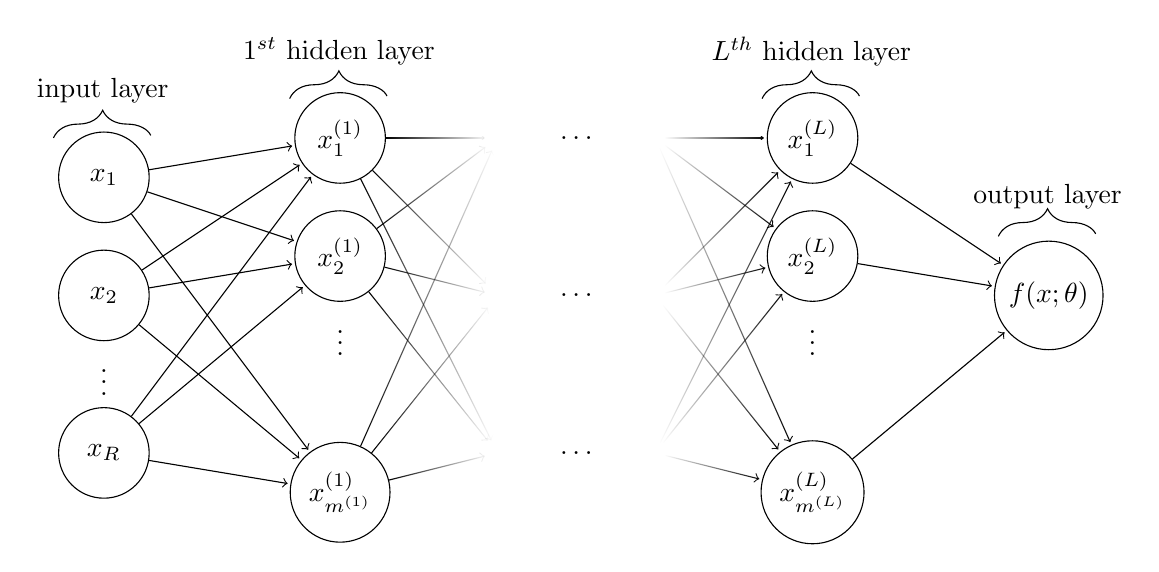
\begin{tikzpicture}[shorten >=1pt]
		\tikzstyle{unit}=[draw,shape=circle,minimum size=1.15cm]
		%\tikzstyle{hidden}=[draw,shape=circle,fill=black!25,minimum size=1.15cm]
		\tikzstyle{hidden}=[draw,shape=circle,minimum size=1.15cm]
 
		\node[unit](x0) at (0,3.5){$x_1$};
		\node[unit](x1) at (0,2){$x_2$};
		\node at (0,1){\vdots};
		\node[unit](xd) at (0,0){$x_R$};
 
		\node[hidden](h10) at (3,4){$x_1^{(1)}$};
		\node[hidden](h11) at (3,2.5){$x_2^{(1)}$};
		\node at (3,1.5){\vdots};
		\node[hidden](h1m) at (3,-0.5){$x_{m^{(1)}}^{(1)}$};
 
		\node(h22) at (5,0){};
		\node(h21) at (5,2){};
		\node(h20) at (5,4){};
		
		\node(d3) at (6,0){$\ldots$};
		\node(d2) at (6,2){$\ldots$};
		\node(d1) at (6,4){$\ldots$};
 
		\node(hL12) at (7,0){};
		\node(hL11) at (7,2){};
		\node(hL10) at (7,4){};
		
		\node[hidden](hL0) at (9,4){$x_1^{(L)}$};
		\node[hidden](hL1) at (9,2.5){$x_2^{(L)}$};
		\node at (9,1.5){\vdots};
		\node[hidden](hLm) at (9,-0.5){$x_{m^{(L)}}^{(L)}$};
 

		\node[unit](y2) at (12,2){$f(x;\theta)$};
 
		\draw[->] (x0) -- (h11);
		\draw[->] (x0) -- (h1m);
		\draw[->] (x0) -- (h10);
 
		\draw[->] (x1) -- (h11);
		\draw[->] (x1) -- (h1m);
		\draw[->] (x1) -- (h10);
 
		\draw[->] (xd) -- (h11);
		\draw[->] (xd) -- (h1m);
 		\draw[->] (xd) -- (h10);
 		
		\draw[->] (hL0) -- (y2);
 
		\draw[->] (hL1) -- (y2);
 
		\draw[->] (hLm) -- (y2);
 
		\draw[->,path fading=east] (h10) -- (h21);
		\draw[->,path fading=east] (h10) -- (h22);
		\draw[->,path fading=east] (h10) -- (h20);
		
		\draw[->,path fading=east] (h11) -- (h21);
		\draw[->,path fading=east] (h11) -- (h22);
		\draw[->,path fading=east] (h11) -- (h20);
		
		\draw[->,path fading=east] (h1m) -- (h21);
		\draw[->,path fading=east] (h1m) -- (h22);
		\draw[->,path fading=east] (h1m) -- (h20);
		
		\draw[->,path fading=west] (hL10) -- (hL0);
		\draw[->,path fading=west] (hL11) -- (hL0);
		\draw[->,path fading=west] (hL12) -- (hL0);
		
		\draw[->,path fading=west] (hL10) -- (hL1);
		\draw[->,path fading=west] (hL11) -- (hL1);
		\draw[->,path fading=west] (hL12) -- (hL1);
		
		\draw[->,path fading=west] (hL10) -- (hLm);
		\draw[->,path fading=west] (hL11) -- (hLm);
		\draw[->,path fading=west] (hL12) -- (hLm);
		
		\draw [decorate,decoration={brace,amplitude=10pt},xshift=-4pt,yshift=0pt] (-0.5,4) -- (0.75,4) node [black,midway,yshift=+0.6cm]{input layer};
		\draw [decorate,decoration={brace,amplitude=10pt},xshift=-4pt,yshift=0pt] (2.5,4.5) -- (3.75,4.5) node [black,midway,yshift=+0.6cm]{$1^{\text{st}}$ hidden layer};
		\draw [decorate,decoration={brace,amplitude=10pt},xshift=-4pt,yshift=0pt] (8.5,4.5) -- (9.75,4.5) node [black,midway,yshift=+0.6cm]{$L^{\text{th}}$ hidden layer};
		\draw [decorate,decoration={brace,amplitude=10pt},xshift=-4pt,yshift=0pt] (11.5,2.75) -- (12.75,2.75) node [black,midway,yshift=0.5cm]{output layer};
	\end{tikzpicture}
	\caption[Multilayer perceptrons with $(L+1)$-layers]{Multilayer perceptrons with $(L+1)$-layers with $P$ input features and 1 output. The $l^{\text{th}}$ hidden layer contains $m^{(l)}$ hidden neurons.}
	\label{fig:multilayer-perceptron}
\end{figure}

So the MLPs is not like classical linear regression in section \ref{LSM} where a single linear transformation from input to output is applied. The unique attribute of neural network is the ability to approximate any kind of function\footnote{Universal Approximate Theorem page 194 \parencite{Goodfellow-et-al-2016}}, because of the flexibility with applying multiple functions to the input layer. The neural network has a lot of different design options, where e.g. hidden layers, layer width, depth, activation functions etc. are hyperparameters. In general it is recommended to use many hidden covariates (neurons) rather than too few. The danger of overfitting is than avoided by introducing some kind of penalty to avoid that the model becomes overly large, which we will discuss further in section \ref{regularization}.\\

To fit a model the model need initialization of weights, biases and activation functions. In order to measure the performance of the model, we need a function to measure the difference between the approximation $f(\bm{x};\bm{\theta})$ and the target values $f^*(\bm{x})$. The function used to quantify this approximation is the loss function, where the cost function is the average over the loss functions. The cost function tells how close the prediction $f(\bm{x};\bm{\theta})$ is to the target y. The cost function is key to improving our model in machine learning lingo training the model, hence the next section will cover model training.

%-----------------------------------
%	SUBSECTION 3
%-----------------------------------
\subsection{Training The Network}\label{trainNetwork}
Training the network is key for building a high quality model. The performance of the model is measured by the cost function, where the cost function used in this thesis is the the empirical risk function.
\begin{align*}
J(\theta)=E_{(\bm{x},y)\sim \hat{p}_{data}} L(f(\bm{x};\bm{\theta)},y)= \frac{1}{k}\sum_{k=1}^{K} L(f(x_k;\theta),y_k)
\end{align*}
The loss function $L$ in empirical risk function for training is chosen to be quadratic, hence for training we penalize with mean square error (MSE) as our cost function.\\

From above we see that the cost function is a way to measure the approximation of $f^*(x)$ by our model $f(\bm{x};\bm{\theta})$. The training is important e.g. imagine after random initialization of parameter and construction of the MLPs we reported the output given the inputs of the model. This model would probably results in a high cost function value and bad performance because the given weights would produce a function that do not fit training data. The way out of the high cost function is to try to minimize the cost function over the weightspace hence training for MLPs is essentially a optimization of a non convex function. Remember the MLPs is a chain of functions (section \ref{architectureMLPs}) where the structure often makes the optimization a non convex problem hence a global minimum is seldom archived. Other pitfalls for optimization of MLPs are weight symmetry, steep cliffs, saddle points, vanishing and exploding gradient.\\

The actual optimization algorithms for MLPs are based on gradients, where we make small local moves. The overall goal is to find $\theta$ to reduce the test error. Within gradient methods there are batch gradient descend and mini-batch stochastic gradient descend, where the former is training on the whole data set, and the latter is only for a subset of the data set. The mini-batch methods have the advantage it can parallelized hence faster training. An epoch is the number of complete data set training cycles to update the weights. For the mini-batching techniques it is important to random sample from the whole data set in order to get unbiased gradient estimation. \\

The goal of the optimization algorithms is to find critical points $\nabla J(\theta)=0$, hence to obtain the critical points the iterative methods move in the opposite direction of sign of derivative $\nabla J(\theta)$. I.e. the gradient tells us how to update the parameters with a stepsize called the learning rate $\eta$:
$$\theta_{new}=\theta_{old} - \eta \nabla J(\theta_{old}) $$
$J(\theta)$ is the cost function, hence remember we use the MSE:
$$J(\theta)= \frac{1}{K}\sum_{k=1}^{K} L(f(x_k;\theta),y_k)=\frac{1}{K}\sum_{k=1}^{K} (y_k-\hat{y}_k)^2$$
Common method to estimate the parameters is gradient descent, stochastic gradient descent (SGD) and Adam, where all the optimization algorithms are iterative. Gradient descend uses the whole batch for each update, where Adam and SGD use mini-batches for each update. The Adam algorithm uses a adaptive learning rate, where the two others use constant or descending learning rate. The Adam method makes greater progress in more gently sloped directions of weightspace compared to SGD and gradient descent. \\

Besides choosing a optimization procedure the initialization of the parameters are important. There is a lot different suggestions to initialize parameters, but there is no general golden rule at the moment because lack of understanding of the optimization procedure in neural nets. Often the practitioners tend to use simple and heuristic methods where it has been shown the initialization breaks weight symmetry.\\

The most common way of finding gradients is the backpropagation algorithm, where the basic idea is the chain rule from calculus.
$$\frac{dz}{dx}= \frac{dz}{dy} \frac{dy}{dx}$$
To understand backpropagation it is often useful with a computational graph created by forward propagation, where the backpropagation compute the derivative from output layer to input layer by going backward in the computational graph. The training process is a forward-backward algorithm. Different starting values of $\theta$ will result in different parameters. The good news is that these predictors typically do not differ by very much. It is recommended to work with a set of different starting values, and then use as a final predictor the average of the individual predictors stemming from each starting value.

%-----------------------------------
%	SUBSECTION 4
%-----------------------------------
\subsection{Regularization}\label{regularization}
The number of parameters and the capacity of neural networks arise often the problem of overfitting, i.e. the model does not generalize well on new data. Regularization is a technique that alter our optimization problem to discourage complex models, hence avoid the problem of overfitting. Some common methods for deep learning are parameter norm regularization, early stopping and dropout.\\

Early stopping is a effective and simple method for regularization. Compared to parameter norm regularization the early stopping algorithm does not harm the learning dynamics. The early stopping method is also computational efficient, hence it makes a popular regularization method for deep learning. The idea of early stopping is that the iterative training algorithm keeps improving the train error, but training too extensively leads the test error to rise. The idea is then to split your data into validation and train data sets, where you determine the best $\hat{\theta}$ and the corresponding training steps $\hat{i}$ by iterative comparing the cost function on the validation set. The algorithm stops after a predefined number of steps without improving the cost function on the validation set. The number of epochs to wait for the cost function not to improve is called the patient for the early stopping algorithm.\\

Like early stopping the dropout method is computationally inexpensive. The idea is to remove neuron randomly at each training loop, i.e. when updating the gradient, each node is kept with probability $p$, independently of each other. To perform dropout a binary mask is sampled independently for each iterations, where the probability $p$ for 1 is another hyperparameter. The goal is to minimize $E_{\bm{\mu}} J(\bm{\theta}, \bm{\mu})$ where $\bm{\mu}$ is the mask. The result of the procedure is more robust features and a regularizing effect on most models.\\

There is a lot of design options for deep learning, where the choices should be specific for the given task. There is a no free lunch theorem for machine learning, which says no model is superior for all tasks (page 114 \parencite{Goodfellow-et-al-2016}). The design for specific tasks are important where training error and test error can be improved by designing the model for the given task. Another aspect is the computational resources i.e. the memory space and computational time. \\

Pricing derivatives with deep learning methods have two clear benefits. The first is computational time, where after a model is trained, then the model is far superior to the methods presented in chapter \ref{Chapter3}. Another advantage is the non-linearities of the model making it possible to fit more complex functions. The application of deep learning in option pricing theory will be explored in next chapter.
